\documentclass[
  a4paper,
  abstract=true,
  twoside,
  listof=totoc,
  numbers=noenddot,
  bibliography=totoc,
  BCOR1.5cm,
  headsepline,
  DIV12,
  appendixprefix,
  final
] {scrreprt}

% You should select either american or british instead of english here:
\usepackage[ngerman,english]{babel}
\usepackage{fontspec}
\usepackage{color}

\usepackage[pdftex,
citebordercolor={0.75 0.75 1},
filebordercolor={0.75 0.75 1},
linkbordercolor={0.75 0.75 1},
% pagebordercolor={0.75 0.75 1},
urlbordercolor={0.75 0.75 1},
pdfborder={0.75 0.75 1},plainpages=false,pdfpagelabels=true]{hyperref}
\hypersetup{%
  pdftitle={Entwicklung einer generischen Kommunikationsschicht für Multi-GPGPU Simulationen am Beispiel PIConGPU},
  pdfauthor={Erik Zenker},
  pdfkeywords={foo, bar},
}

\usepackage[backend=biber,style=alphabetic,alldates=long]{biblatex}

\usepackage{varioref}           % nice refs
\usepackage{csquotes}
\usepackage{graphicx}           % graphics
\usepackage{caption}            % manipulate fugures
\usepackage{subcaption}         % allow for subfigures
\usepackage{listings}           % nice source code listings
\usepackage{color}
\usepackage{booktabs}           % nice tables
\usepackage{microtype}          % better looking text borders
\usepackage{units}              % unified way of setting values with units
\usepackage{array}
\usepackage{fancybox}           % provide nice boxes
\usepackage{units}              % unified way of setting values with units
\usepackage{fancyvrb}           % algorithm-boxes
\usepackage{pdfpages}
\usepackage{hyphenat}
\usepackage{todonotes}
\usepackage{xspace}
\usepackage{setspace}

% use this one last
% (redefines some macros for compatibility with KOMAScript)
\usepackage{scrhack}

\addbibresource{own.bib}
 
\definecolor{mygreen}{rgb}{0,0.6,0}
\definecolor{mygray}{rgb}{0.5,0.5,0.5}
\definecolor{mymauve}{rgb}{0.58,0,0.82}
 
% Biblatex Style
\setcounter{secnumdepth}{3}     % limit enumeration depth
\setcounter{tocdepth}{1}        % limit TOC depth

% Listing Style

\lstset{ %
  frame=shadowbox,
  rulesepcolor=\color{blue},
  backgroundcolor=\color{white},   % choose the background color; you must add \usepackage{color} or \usepackage{xcolor}
%  basicstyle=\footnotesize,        % the size of the fonts that are used for the code
  breakatwhitespace=false,         % sets if automatic breaks should only happen at whitespace
  breaklines=true,                 % sets automatic line breaking
  captionpos=b,                    % sets the caption-position to bottom
  commentstyle=\color{mygreen},    % comment style
  deletekeywords={...},            % if you want to delete keywords from the given language
  escapeinside={\%*}{*)},          % if you want to add LaTeX within your code
  extendedchars=true,              % lets you use non-ASCII characters; for 8-bits encodings only, does not work with UTF-8
  frame=single,                    % adds a frame around the code
  keepspaces=true,                 % keeps spaces in text, useful for keeping indentation of code (possibly needs columns=flexible)
  keywordstyle=\color{blue},       % keyword style
  language=C,                 % the language of the code
 % morekeywords={*,...},            % if you want to add more keywords to the set
  numbers=left,                    % where to put the line-numbers; possible values are (none, left, right)
  numbersep=7pt,                   % how far the line-numbers are from the code
  numberstyle=\tiny\color{mygray}, % the style that is used for the line-numbers
  rulecolor=\color{black},         % if not set, the frame-color may be changed on line-breaks within not-black text (e.g. comments (green here))
  showspaces=false,                % show spaces everywhere adding particular underscores; it overrides 'showstringspaces'
  showstringspaces=false,          % underline spaces within strings only
  showtabs=false,                  % show tabs within strings adding particular underscores
  stepnumber=1,                    % the step between two line-numbers. If it's 1, each line will be numbered
  stringstyle=\color{mymauve},     % string literal style
  tabsize=2,                       % sets default tabsize to 2 spaces
  title=\lstname                   % show the filename of files included with \lstinputlisting; also try caption instead of title
}

% Typesetting options
\tolerance 2414
\hbadness 2414
\emergencystretch 1.5em
\hfuzz 0.3pt
\widowpenalty=10000     % Hurenkinder
\clubpenalty=10000      % Schusterjungen
\vfuzz \hfuzz
\raggedbottom

% use nice footnote indentation
\deffootnote[1em]{1em}{1em}{\textsuperscript{\thefootnotemark}\,}
 
% some common commands
\newcommand{\drops}{\texorpdfstring{\textsc{Drops}\xspace}{DROPS}}

\newcommand{\expr}[1]{\textcolor{blue}{#1}}


% If you know when you will hand in your thesis, enter the date here.
%\date{30. April 2009}
%\newcommand{\printdate}{\@date}

\begin{document}

\pagenumbering{Roman}

 
\selectlanguage{ngerman}

\begin{singlespace}

\subject{{\LARGE Diplomarbeit}}

\title{Entwicklung einer generischen Kommunikationsschicht für Multi-GPGPU Simulationen am Beispiel PIConGPU}

\author{Erik Zenker}

\publishers{Technische Universität Dresden\\
Fakultät Informatik\\
Institut für Systemarchitektur\\
Professur für Rechnerarchitektur\\
\begin{minipage}{\textwidth}%\\
\vskip 6cm
 {\normalsize }\begin{tabular}{ll}
Betreuender Hochschullehrer: &
Prof. Dr. Wolfgang E. Nagel\tabularnewline
Betreuender Mitarbeiter: &
Dr. Guido Juckeland\tabularnewline
\end{tabular} {\normalsize }\end{minipage}}

\maketitle
\end{singlespace}

\cleardoublepage



\includepdf{images/diplom-aufgabe.pdf}
\cleardoublepage

 
\selectlanguage{ngerman}

\section*{\vfill{} \thispagestyle{empty}
Erklärung}

Hiermit erkläre ich, dass ich diese Arbeit selbstständig erstellt
und keine anderen als die angegebenen Hilfsmittel benutzt habe.
\bigskip{}

\noindent Dresden, den \today % \printdate % if you defined date earlier
\vspace{2.5cm}

\noindent Otto Mustermann \cleardoublepage{}

% NOTE: if you selected british or american above, change that here too
\selectlanguage{english}

\begin{abstract}
% -*- Mode: Latex -*-

%  Zusammenfassung

% Zu einer runden Arbeit gehört auch eine Zusammenfassung, die
% eigenständig einen kurzen Abriß der Arbeit gibt. Eine halbe bis ganze
% DINA4 Seite ist angemessen. Dafür läßt sich keine Gebrauchsanweisung
% geben (für irgendetwas müssen die Betreuer ja auch noch da
% sein).

\ldots abstract \ldots

\todo{write abstract}

%%% Local Variables:
%%% TeX-master: "diplom"
%%% End:



\end{abstract}

\cleardoublepage

\tableofcontents

\cleardoublepage

% remove this on final
\listoftodos
\cleardoublepage

\listoffigures
\cleardoublepage

\listoftables
\cleardoublepage

\pagenumbering{arabic}
\chapter{Introduction}
\label{sec:intro}

% Die Einleitung schreibt man zuletzt, wenn die Arbeit im Großen und
% Ganzen schon fertig ist. (Wenn man mit der Einleitung beginnt - ein
% häufiger Fehler - braucht man viel länger und wirft sie später doch
% wieder weg). Sie hat als wesentliche Aufgabe, den Kontext für die
% unterschiedlichen Klassen von Lesern herzustellen. Man muß hier die
% Leser für sich gewinnen. Das Problem, mit dem sich die Arbeit befaßt,
% sollte am Ende wenigsten in Grundzügen klar sein und dem Leser
% interessant erscheinen. Das Kapitel schließt mit einer Übersicht über
% den Rest der Arbeit. Meist braucht man mindestens 4 Seiten dafür, mehr
% als 10 Seiten liest keiner.

\todo{adopt title page}

\todo{adopt disclaimer}

\todo{write introduction}

\section{A Section}

Referencing other chapters: \ref{sec:state} \ref{sec:design}
\ref{sec:implementation} \ref{sec:evaluation} \ref{sec:futurework}
\ref{sec:conclusion}

\begin{table}[htp]
  \centering
  \begin{tabular}{lrr}
    \textbf{Name} & \textbf{Y} & \textbf{Z} \\
    \hline
    \textit{Foo} & 20,614 & \unit[23]{\%} \\
    \textit{Bar} & 9,914 & \unit[11]{\%} \\
    \textit{Foo + Bar} & 30,528 & \unit[34]{\%} \\
    \hline
    \textit{total} & 88,215 & \unit[100]{\%} \\

  \end{tabular}
  \caption[Some interesting numbers]{Various very important looking numbers and sums.}
  \label{tab:numbers}
\end{table}

More text referencing Table~\ref{tab:numbers}.

\section{Another Section}

\begin{figure}[tbp]
  \centering
  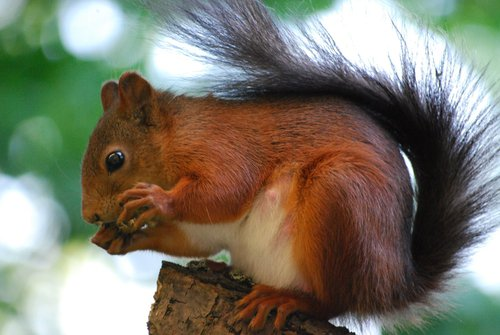
\includegraphics[width=0.8\textwidth]{images/squirrel}
  \caption[Short description]{A long description of this squirrel figure.
  Image taken from
  \url{http://commons.wikimedia.org/wiki/File:Sciurus-vulgaris_hernandeangelis_stockholm_2008-06-04.jpg}}
  \label{fig:squirrel}
\end{figure}

Citing \cite{bellard2005qfa} other documents \cite{bellard2005qfa, boileau06}
and Figure~\ref{fig:squirrel}.

Something with umlauts and a year/month date:
\cite{becher04:_feurig_hacken_mit_firew}.

And some online resources: \cite{green04}, \cite{patent:4819234}

\section{Yet Another Section}

\todo{add content}

\begin{figure}[tbp]
 \missingfigure{Come up with a mindblowing figure.}
 \caption{A mindblowing figure}
 \label{fig:todo}
\end{figure}

\section{Test commands}

\texttt{memcpy}
A sentence about BASIC. And a correctly formatted one about ECC\@.

\cleardoublepage

%%% Local Variables:
%%% TeX-master: "diplom"
%%% End:

\chapter{Technical Background}
\label{sec:state}

% Hier werden zwei wesentliche Aufgaben erledigt:

% 1. Der Leser muß alles beigebracht bekommen, was er zum Verständnis
% der späteren Kapitel braucht. Insbesondere sind in unserem Fach die
% Systemvoraussetzungen zu klären, die man später benutzt. Zulässig ist
% auch, daß man hier auf Tutorials oder Ähnliches verweist, die hier auf
% dem Netz zugänglich sind.

% 2. Es muß klar werden, was anderswo zu diesem Problem gearbeitet
% wird. Insbesondere sollen natürlich die Lücken der anderen klar
% werden. Warum ist die eigene Arbeit, der eigene Ansatz wichtig, um
% hier den Stand der Technik weiterzubringen? Dieses Kapitel wird von
% vielen Lesern übergangen (nicht aber vom Gutachter ;-), auch später
% bei Veröffentlichungen ist "Related Work" eine wichtige Sache.

% Viele Leser stellen dann später fest, daß sie einige der Grundlagen
% doch brauchen und blättern zurück. Deshalb ist es gut,
% Rückwärtsverweise in späteren Kapiteln zu haben, und zwar so, daß man
% die Abschnitte, auf die verwiesen wird, auch für sich lesen
% kann. Diese Kapitel kann relativ lang werden, je größer der Kontext
% der Arbeit, desto länger. Es lohnt sich auch! Den Text kann man unter
% Umständen wiederverwenden, indem man ihn als "Tutorial" zu einem
% Gebiet auch dem Netz zugänglich macht.

% Dadurch gewinnt man manchmal wertvolle Hinweise von Kollegen. Dieses
% Kapitel wird in der Regel zuerst geschrieben und ist das Einfachste
% (oder das Schwerste weil erste).

%%%%%%%%%%%%%%%%%%%%%%%%%%%%%%%%%%%%%%%%%%%%%%%%%%%%%%%%%%%%%%%%%%%%%%%%%%%%%%%%
%                                                                              %
% TECHNICAL BACKGROUND                                                         %
%                                                                              %
%%%%%%%%%%%%%%%%%%%%%%%%%%%%%%%%%%%%%%%%%%%%%%%%%%%%%%%%%%%%%%%%%%%%%%%%%%%%%%%%



%%%%%%%%%%%%%%%%%%%%%%%%%%%%%%%%%%%%%%%%%%%%%%%%%%%%%%%%%%%%%%%%%%%%%%%%%%%%%%%%
%                                                                              %
% HIGH PERFORMANCE COMPUTING                                                   %
%                                                                              %
%%%%%%%%%%%%%%%%%%%%%%%%%%%%%%%%%%%%%%%%%%%%%%%%%%%%%%%%%%%%%%%%%%%%%%%%%%%%%%%%
\section{Cluster computing}
Parallel computers are not anymore specialized traditional
supercomputing platforms, instead low cost off-the-shelf commodity
computers form so called compute clusters \cite{ref:hpcc1}.

These loosely coupled components of a cluster are built from
multiprocessor PCs or workstation and are connected via a high-speed
network connection.

Therefore a compute cluster forms a homogeneous network of compute
entities, which are also called nodes. Every node can consist out of
different compute devices such as multicore CPUs and with more and
more popularity also acceleration devices like graphic cards. With the
consequence of a hierarchicle structure on the node with non-uniform
memory access (NUMA) \cite[numa]{ref:numa}.

The memory between nodes is not shared in principle, thus normally
every node has its own memory and therfore a compute cluster belongs
to the class of distributed memory architectures.

Only a few problems can be calculated without exchanging information
between other nodes. Thus each node has the challange to retrieve all
the data, that is needed to calculate the next step of its
computation.

\begin{itemize}
\item Computational power of single computer are limited by 
  phsical laws
\item Computers of a cluster need to work together
\item Future of high performance computing \cite{ref:hpc}
\item Scales
\end{itemize}

There are several ways to retrieve data from other nodes. The most
obvious way is to use direct communication between nodes. This can be
very low level protocols like TCP, UDP, IP by using UNIX sockets
(\ref{sec:tcp_udp_ip}) or more modern and abstract models like the
message passing interface (\ref{sec:mpi}) and the parallel virual
machine (\ref{sec:pvm}).These traditional ways to communicate in
cluster systems will be discussed in section \ref{sec:communication}.

\todo{More related work + references to distributed shared memory} An
other way is to create a layer on top of the all cluster nodes, so
that the cluster looks like a single machine with a lot of devices and
a shared memory. This is called a distributed shared memory
architecture. The layer can be adjusted to the needs of the user.  It
can be an own operating system like MOSIX \cite{ref:mosix}, some
virtualisation layer \cite{ref:cluster_virt} etc.  This kind of data
exchange between nodes will not be discussed in detail in this thesis.
\begin{itemize}
\item Usage of simple parallization schemas like OpenMP, Pthreads
\item No explicit communication necessary
\item Easy usage for non computer scientists
\item higher abstraction \rightarrow loose of control and efficiency
\end{itemize}


%%%%%%%%%%%%%%%%%%%%%%%%%%%%%%%%%%%%%%%%%%%%%%%%%%%%%%%%%%%%%%%%%%%%%%%%%%%%%%%%
%                                                                              %
% TRADITIONAL COMMUNICATION MECHANISMS IN CLUSTER SYSTEMS                      %
%                                                                              %
%%%%%%%%%%%%%%%%%%%%%%%%%%%%%%%%%%%%%%%%%%%%%%%%%%%%%%%%%%%%%%%%%%%%%%%%%%%%%%%%
\section{Traditional communication mechanisms in cluster systems}
\label{sec:communication}


\subsection{IP,TCP, UDP, Sockets}
\label{sec:tcp_udp_ip}
\begin{itemize}
  \item Communication in the UNIX way
  \item IP, Internet Protocol was there before LAN and clusters \cite{ref:ip}
  \item TCP and UDP on top of IP (TCP/IP, UDP/IP) \cite{ref:tcp, ref:udp}
  \item TCP/IP and UDP/IP where made available through Berkeley Sockets \cite{ref:sockets}
  \item Sockets where designed by the UNIX philosophie; everything is a file (file descriptors)
  \item Sockets where not designed with the usage in hpc environment in mind
\end{itemize}

\subsection{Message passing intferface (MPI)}
\label{sec:mpi}

The message passing interface (MPI) is a standardized and portable
message-passing specification, specified by the Message Passing
Interface Forum \cite{ref:mpi_specification} and has become
the de facto standard for communication in cluster systems. 

Implementations are available on virtually every parallel computer systems.
Popular implementations are MPICH and Open MPI. MPICH2 implements the
MPI-2.1 specification. Open MPI has the goal to be full MPI-3 standard conform.

The first version of the specification, known as MPI-1, was completed
in 1994 making use of the most attractive features of allready
existing message passing systems.  Further improvements followed 1997
by version MPI-2 and 2008 by version MPI-3. There might be some
confusion about the several MPI specification versions. Major versions
like MPI-2 or MPI-3 come with new features to the MPI standard and
minor versions like MPI-1.1 or MPI-1.2 come with clarifiacations of
allready existing features.  In the following the key features of the
varying MPI versions are listed:

\begin{itemize}
  \item MPI-1 (1994)
    \begin{itemize}
      \item Basix point-to-point communication
      \item Collectives
      \item Derived datatypes
    \end{itemize}
  \item MPI-2 (1997)
    \begin{itemize}
      \item Parallel I/O
      \item Remote memory operations (one-sided)
      \item Dynamic process management
    \end{itemize}
  \item MPI-3 (1998)
    \begin{itemize}
      \item Nonblocking collectives
      \item Improved one-sided communication interface
    \end{itemize}
\end{itemize}

An MPI programm is a set of autonomous processes, executing their own
code, in an MIMD style \cite{Flynn:1972:COE:1952456.1952459}. Each
process rests in his own adress space and communicates via MPI
communication primitives with other processes in the same MPI
programm. 

Processes are identified according to their relative rank in a group by
consecutive integers from 0 to groupsizie-1. Which the initial group
compromises the full set of processes with ranks in the range 0 to 
the number of processes. A typical MPI program run is composed from
the following steps:

\begin{itemize}
  \item MPI process
    \begin{enumerate}
      \item Start MPI programm
      \item Init MPI environment
      \item Ask for own rank
      \item Ask for number of ranks overall
      \item Depend on own rank and overall ranks do some task (varying flow of control between ranks)
      \item Communicate with other ranks
      \item Finalize MPI environment
      \item Exit MPI programm
    \end{enumerate}
\end{itemize}

MPI provides a large and versatile set of routines. At its most
basic, MPI has functions for sending and receiving a message.
These functions are available both blocking and nonblocking.

Further a variaty of collective operations that involve
a group of processes are defined. All members of the group
have to paticipate to sucessfully execute the collective operation.
The result of the operation is either received by one process,
the so called root, or by all processes of a group.

The MPI communication is implemented on top of existing communication
abstractraction provided by the underlying cluster system (sockets, AM, etc.)



\begin{itemize}
\item Fits needs of parallel programming community
\item low latency, high bandwidth
\item Zero-data copy transfer
\item Free libraries available (OpenMPI)
\item Language independent communication protocol
\end{itemize}

\subsection{Parallel virtual machine (PVM)}
\label{sec:pvm}
\begin{itemize}
\item Parallel Virtual Machine connects a collection of heterogeneous computers
  to a single "parallel virtual machine"
  (http://en.wikipedia.org/wiki/PVM)
\item Support for communication and synchronization operations
\item Configuration control
\item synamic Spawning of pocressen
\item PVM daemons are spawned on a set of nodes
\item Local processes connect to PVM daemons and can 
  communicate through this daemon to other PVM daemons
\end{itemize}

\section{Fault tolerance}
\section{Load balancing}

%%%%%%%%%%%%%%%%%%%%%%%%%%%%%%%%%%%%%%%%%%%%%%%%%%%%%%%%%%%%%%%%%%%%%%%%%%%%%%%%
%                                                                              %
% PIConGPU - THE APPLICATION                                                   %
%                                                                              %
%%%%%%%%%%%%%%%%%%%%%%%%%%%%%%%%%%%%%%%%%%%%%%%%%%%%%%%%%%%%%%%%%%%%%%%%%%%%%%%%
\section{PIConGPU - the application}
\label{sec:picongpu}
\begin{itemize}
  \item A Many-GPGPU Particle-in-Cell Code
  \item Electric and magnetic fields are interpolated on a physical
    grid dividing the simulated volume into cells
  \item Simulated volume divided in cubes / squares
  \item Every GPU computes one of these cubes / squares
  \item One MPI process per cube square
  \item Offload of simulation data to GPUs
  \item Communication based on MPI
\end{itemize}

\subsection{Requirements for the upcoming generation of super computers}
\begin{itemize}
\item Run picongpu on xeon phi in native mode
\item Exchangeable communication layer to be portable / ready  for the upcoming
  generation of acceleration devices
\end{itemize}

\subsection{Communication topologie}
\begin{itemize}
\item 3- or 2-dimensional mesh
\item next neighbor communication
\item Some collective operations (Allgather, Gather, GatherV, AllReduce, Reduce
\item Offload of simulation data to GPU
\end{itemize}


\cleardoublepage

%%% Local Variables:
%%% TeX-master: "diplom"
%%% End:

\chapter{Design}
\label{sec:design}

% Ist das zentrale Kapitel der Arbeit. Hier werden das Ziel sowie die
% eigenen Ideen, Wertungen, Entwurfsentscheidungen vorgebracht. Es kann
% sich lohnen, verschiedene Möglichkeiten durchzuspielen und dann
% explizit zu begründen, warum man sich für eine bestimmte entschieden
% hat. Dieses Kapitel sollte - zumindest in Stichworten - schon bei den
% ersten Festlegungen eines Entwurfs skizziert werden.
% Es wird sich aber in einer normal verlaufenden
% Arbeit dauernd etwas daran ändern. Das Kapitel darf nicht zu
% detailliert werden, sonst langweilt sich der Leser. Es ist sehr
% wichtig, das richtige Abstraktionsniveau zu finden. Beim Verfassen
% sollte man auf die Wiederverwendbarkeit des Textes achten.

% Plant man eine Veröffentlichung aus der Arbeit zu machen, können von
% diesem Kapitel Teile genommen werden. Das Kapitel wird in der Regel
% wohl mindestens 8 Seiten haben, mehr als 20 können ein Hinweis darauf
% sein, daß das Abstraktionsniveau verfehlt wurde.

\section{A Graph-based communication layer}

\cleardoublepage

%%% Local Variables:
%%% TeX-master: "diplom"
%%% End:

\chapter{Implementation}
\label{sec:implementation}

% Hier greift man einige wenige, interessante Gesichtspunkte der
% Implementierung heraus. Das Kapitel darf nicht mit Dokumentation oder
% gar Programmkommentaren verwechselt werden. Es kann vorkommen, daß
% sehr viele Gesichtspunkte aufgegriffen werden müssen, ist aber nicht
% sehr häufig. Zweck dieses Kapitels ist einerseits, glaubhaft zu
% machen, daß man es bei der Arbeit nicht mit einem "Papiertiger"
% sondern einem real existierenden System zu tun hat. Es ist sicherlich
% auch ein sehr wichtiger Text für jemanden, der die Arbeit später
% fortsetzt. Der dritte Gesichtspunkt dabei ist, einem Leser einen etwas
% tieferen Einblick in die Technik zu geben, mit der man sich hier
% beschäftigt. Schöne Bespiele sind "War Stories", also Dinge mit denen
% man besonders zu kämpfen hatte, oder eine konkrete, beispielhafte
% Verfeinerung einer der in Kapitel 3 vorgestellten Ideen. Auch hier
% gilt, mehr als 20 Seiten liest keiner, aber das ist hierbei nicht so
% schlimm, weil man die Lektüre ja einfach abbrechen kann, ohne den
% Faden zu verlieren. Vollständige Quellprogramme haben in einer Arbeit
% nichts zu suchen, auch nicht im Anhang, sondern gehören auf Rechner,
% auf denen man sie sich ansehen kann.

\ldots implementation \ldots

\todo{write implementation}

\cleardoublepage

%%% Local Variables:
%%% TeX-master: "diplom"
%%% End:

\chapter{Evaluation}
\label{sec:evaluation}

% Zu jeder Arbeit in unserem Bereich gehört eine Leistungsbewertung. Aus
% diesem Kapitel sollte hervorgehen, welche Methoden angewandt worden,
% die Leistungsfähigkeit zu bewerten und welche Ergebnisse dabei erzielt
% wurden. Wichtig ist es, dem Leser nicht nur ein paar Zahlen
% hinzustellen, sondern auch eine Diskussion der Ergebnisse
% vorzunehmen. Es wird empfohlen zunächst die eigenen Erwartungen
% bezüglich der Ergebnisse zu erläutern und anschließend eventuell
% festgestellte Abweichungen zu erklären.

\ldots evaluation \ldots

\todo{write evaluation}

\cleardoublepage

%%% Local Variables:
%%% TeX-master: "diplom"
%%% End:

\chapter{Future Work}
\label{sec:futurework}

\ldots future work \ldots

\todo{write future work}

\cleardoublepage

%%% Local Variables:
%%% TeX-master: "diplom"
%%% End:

\chapter{Conclusion And Outlook}
\label{sec:conclusion}

%  Schlußfolgerungen, Fragen, Ausblicke

% Dieses Kapitel ist sicherlich das am Schwierigsten zu schreibende. Es
% dient einer gerafften Zusammenfassung dessen, was man gelernt hat. Es
% ist möglicherweise gespickt von Rückwärtsverweisen in den Text, um dem
% faulen aber interessierten Leser (der Regelfall) doch noch einmal die
% Chance zu geben, sich etwas fundierter weiterzubilden. Manche guten
% Arbeiten werfen mehr Probleme auf als sie lösen. Dies darf man ruhig
% zugeben und diskutieren. Man kann gegebenenfalls auch schreiben, was
% man in dieser Sache noch zu tun gedenkt oder den Nachfolgern ein paar
% Tips geben. Aber man sollte nicht um jeden Preis Fragen, die gar nicht
% da sind, mit Gewalt aufbringen und dem Leser suggerieren, wie
% weitsichtig man doch ist. Dieses Kapitel muß kurz sein, damit es
% gelesen wird.

\ldots conclusion \ldots

\todo{write conclusion}

\cleardoublepage

%%% Local Variables:
%%% TeX-master: "diplom"
%%% End:


\appendix

%\addchap{Glossar}

% makeglossaries diplom
%\printglossary[style=altlist]
%\printglossary[type=\acronymtype,style=long]

\printbibliography
\iffalse
    % an aid for Kile autocompletion
\bibliography{own.bib}
\fi

\end{document}
